\section{\limdds are exponentially more succinct than \qmdds}
\label{sec:exponential-separations}
%\todo[inline]{Vedran:     Sec 4: not what I would expect to read as the first sentence  -0 title says QMDDs... sentence does not mention them but talks about stabilizers... clarify.
%	Maybe: the goal of this section is to prove that... [btw.. if that is the goal, why is this not the title? aha.. because that is the ultimate goal? Then: one of the main goals of the paper is to shiw that.. in order to do so we first show.. but now I see you say "this section shows a stronger result". so I think the first sentence is not what you want}

%In the following sections, we show that LIMDDs can efficiently represent (this section) and manipulate (sec.~\ref{sec:quantum-simulation}) a strict superset of all stabilizer states.
In this section, we show that \limdds can be exponentially more succinct than the union of \qmdds and stabilizer states (\autoref{thm:limdd-superset-qmdd-plus-stabilizers}).
Namely, we show that polynomial-sized $G$-\limdds can represent stabilizer states, using $G=\textsf{Pauli}$, (\autoref{thm:pauli-limdd-is-stabilizer}) whereas \qmdds require exponential space to represent cluster states (\autoref{thm:graph-state-qmdd-lower-bound}).
In \autoref{sec:graph-state-lower-bound} and \autoref{sec:graph-states-limdds}, we show that \limdds retain this exponential advantage even when we use the parameter $G=\braket{Z}$ or $G=\braket{X}$.\footnote{Note that the proofs in this section do not rely on the specialized definition of reduced \limdds, but only on the parametrized \autoref{def:limdd}.}
We emphasize that this section regards \emph{representation} of quantum states; in \autoref{sec:quantum-simulation}, we show that by using \limdds to represent quantum states, we can \emph{simulate} quantum circuits.

\begin{wrapfigure}{r}{9cm}
    \vspace{-1em}
%    \begin{centering}
	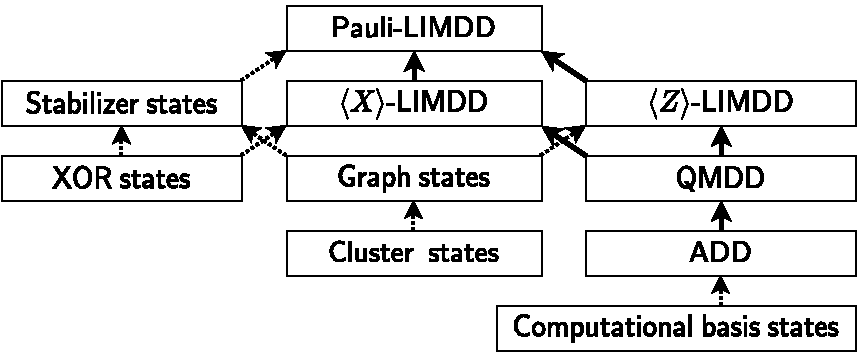
\includegraphics[width=0.55\textwidth]{pics/complexity-inclusion-diagram-no-torus.pdf}
	\caption{
	    \label{fig:complexity-classes-inclusion-diagram}
        Relations between classes of quantum states and families of polynomial-size decision diagrams.
        Every arrow denotes a strict inclusion of sets; in particular, each solid arrow $D_1\to D_2$ denotes an exponential separation between two decision diagram families, i.e., some quantum states have polynomial-size diagrams of type $D_2$, but have only exponential-size diagrams of type $D_1$. The dotted arrows represent inclusion.
%        \todo[inline]{remove DT}
    }
    %\vspace{-1em}
%    \end{centering}
\end{wrapfigure}

\autoref{fig:complexity-classes-inclusion-diagram} visualizes the results from this section.
The boxes with $\braket{Z}$-\limdd denote the \limdd with parameter \mbox{$G=\braket{Z}$}, i.e., \limdds where the labels on edges are all of the form \mbox{$\lambda P_n\otimes\cdots\otimes P_1$} where \mbox{$P_j\in \{\mathbb I, Z\}$}.
Although of course every $\braket{Z}$-\limdd is a Pauli-\limdd, this parameterization is interesting in its own right because it requires only polynomial size to represent any graph state.
Similarly, the $\braket{X}$-\limdd can succinctly represent a set of stabilizer states we call ``XOR states.''
\autoref{sec:graph-states-limdds} proves these results, and proves that \qmdds require exponential size for all these states. 
%Namely, we show that $\braket{Z}$-\limdds can represents graph states (\autoref{thm:z-limdd-is-graph-state}), and that $\braket{X}$-\limdds can represent so-called ``XOR-states'' (\autoref{thm:x-limdd-is-hyperplane}).




\begin{theorem}[Exponential separation between Pauli-\limdd versus QMDD union stabilizer states]
	\label{thm:limdd-superset-qmdd-plus-stabilizers}
	The set of quantum states represented by polynomial-size Pauli-\limdds is a strict superset of the union of stabilizer states and polynomial-size \qmdds.
\end{theorem}
\begin{proof}
    Each $n$-qubit stabilizer state can be represented by a Pauli-\limdd of $n$ nodes (\autoref{thm:pauli-limdd-is-stabilizer}).
    Moreover, if a state has a polynomial-size \qmdd, it also has a polynomial-size \limdd, due to our earlier remark that a \qmdd can be seen as a \glimdd with $G=\set{\mathbb I}$, i.e., each label is of the form $\lambda\mathbb I$ with $\lambda\in\mathbb C$.
%    This shows that the union of stabilizer states and polynomial-size QMDDs is included in the set of polynomial-sizee Pauli-\limdds.
    To show that polynomial-size Pauli-\limdds represent strictly more than these two classes of states, consider $\ket{\phi}:= \ket{T}\otimes \ket{G_n}$, where $\ket{T}=\ket{0}+e^{i\pi/4}\ket{1}$, and where $\ket{G_n}$ is the graph state on the $n\times n$ grid.
    We note that $\ket{\phi}$ is not a stabilizer state, because each computational-basis coefficient of a stabilizer state is of the form $z\cdot 1/\sqrt{2}^k$ for $z\in \{\pm 1, \pm i\}$ and some integer $k\geq 1$ \cite{nest2005local}, while $\bra{1}\otimes \bra{0}^{\otimes n} \ket{\phi} = e^{i\pi/4} \cdot \frac{1}{\sqrt{2}}^n$ is not of this form.
    Moreover, its canonical \qmdd is a root node $\lnode{1}{v_G}{e^{i\pi/4}}{v_G}$ where $v_G$ is the root node of the QMDD for $\ket{G_n}$, which has exponential size (\autoref{thm:graph-state-qmdd-lower-bound}).
    In contrast, the reduced Pauli-\limdd for $\ket{G_n}$ (with root node $w_G$) has $n$ nodes (because $\ket{G_n}$ is a stabilizer state), and hence a polynomial-size Pauli-\limdd for $\ket{T} \otimes \ket{G_n}$ has root node with $\lnode{\unit}{v_G}{e^{i\pi/4} \unit}{v_G}$.
\end{proof}


%In the following proofs, we  use a subset of \limdds, called Tower \limdds formalized in \autoref{def:tower}.
%\begin{definition}[Tower \glimdd]
%    \label{def:tower}
%	A \glimdd is called a Tower \glimdd if it has one node in each layer, i.e., if, for each node, both outgoing edges point to the same target (although these edges may have different labels).
%\end{definition}
%
%\autoref{thm:pauli-limdd-is-stabilizer} characterizes the Tower Pauli-\limdds.
%It is stated here informally; for details and a proof, see \autoref{sec:proof-stabilizer-states-tower-limdds}

Now we give the two statements leading up to \autoref{thm:limdd-superset-qmdd-plus-stabilizers}: \pauli-\limdds represent stabilizer states succinctly (\autoref{thm:pauli-limdd-is-stabilizer}) but \qmdds representing stabilizer states are necessarily large (\autoref{thm:graph-state-qmdd-lower-bound}).
In this theorem, by a Tower \limdd we mean a \limdd which has a single node on each level.

\begin{theorem}[Tower Pauli-\limdds are stabilizer states]
	\label{thm:pauli-limdd-is-stabilizer}
    Let $n>0$.
    Each $n$-qubit stabilizer state is represented by a reduced Tower Pauli-\limdd on $n$ nodes with high edge label factors $\in \{0, \pm 1, \pm i\}$.
	Conversely, every such \limdd represents a stabilizer state.
\end{theorem}
\begin{proof}[Proof sketch]
    We sketch here why each stabilizer state is represented by a reduced Tower Pauli-\limdd and give a full proof in \autoref{thm:pauli-tower-limdds-are-stabilizer-states}.
    Let $\ket{\psi}$ be a stabilizer state.
    If $\ket{\psi} = \ket{x}\ket{\psi'}$ for some $x\in \{0, 1\}$ and $\ket{\psi'}$, then $\ket{\psi'}$ is a stabilizer state and it is represented by a Tower Pauli-\limdd which has a root node with a low edge label $\id$, high edge label $0$ and root edge labelled $X^x \otimes \id$, to the root node of the Tower Pauli-\limdd of $\ket{\psi'}$.
	Otherwise, $\ket{\psi}\propto \ket{0}\ket{\psi_0}+\ket{1}\ket{\psi_1}$, where both $\ket{\psi_0}$ and $\ket{\psi_1}$ are stabilizer states.
    Moreover, if $\ket{\psi}$ is a stabilizer state, there is always a set of single-qubit Pauli gates $P_1,\ldots, P_n$ and a $\lambda \in \{\pm 1, \pm i\}$ such that $\ket{\psi_1}=\lambda P_n\otimes\cdots\otimes P_1\ket{\psi_0}$.
	That is, in our terminology, the states $\ket{\psi_0}$ and $\ket{\psi_1}$ are \emph{isomorphic}.
	Hence $\ket{\psi}$ can be written as
	\begin{align}
		\ket{\psi}=\ket{0}\ket{\psi_0} + \lambda \ket{1}\otimes \left(P_n\otimes\cdots\otimes P_1\ket{\psi_0}\right)
	\end{align}
	This expression suggests the following representation as a Tower Pauli-\limdd: the root node represents $\ket{\psi}$, both its outgoing edges point to a node representing $\ket{\psi_0}$, and its high edge is labeled with the isomorphism $\lambda P_n\otimes\cdots\otimes P_1$; this strategy is then applied recursively to $\ket{\psi_0}$ and its two subfunctions.
    This procedure yields a semi-reduced Tower-Pauli-\limdd, which can be made reduced by making all high labels canonical, from bottom to top.
\end{proof}

\begin{lemma}
	\label{thm:graph-state-qmdd-lower-bound}
	Denote by $\ket{G_n}$ the graph state on the $n \times n$ lattice.
	Each \qmdd representing the cluster state $\ket{G_n}$ has at least $2^{\floor{n/12}}$ nodes.
\end{lemma}
\begin{proof}[Proof sketch]
	Consider a partition of the vertices of the $n\times n$ lattice into two sets $S$ and $T$ of size $\frac{1}{2}n^2$, corresponding to the first $\frac{1}{2}n^2$ qubits under some variable order.
	Then there are at least $\lfloor n/3 \rfloor$ vertices in $S$ that are adjacent to a vertex in $T$ \cite[Th. 11]{lipton1979generalized}.
	Because the degree of the nodes is small, many vertices on this boundary influence the amplitude function independently of one another.
	From this independence, it follows that, for any variable order,
	the partial assignments $\vec a \in \set{0,1}^{\frac{1}{2}n^2}$ induce
	$2^{\lfloor n/12 \rfloor}$ different subfunctions $f_{\vec a}$, where
	$f\colon \set{0,1}^{n^2} \rightarrow \mathbb C$
	is the amplitude function of $\ket{G_n}$.
	The lemma follows by noting that a \qmdd has a single node per unique subfunction modulo phase.
	For details see \autoref{sec:graph-state-lower-bound}.
\end{proof}

%In \autoref{sec:proof-stabilizer-states-tower-limdds}, we characterize Tower $\braket{Z}$-\limdds (\autoref{thm:z-limdd-is-graph-state}) and Tower $\braket{X}$-\limdds (\autoref{thm:x-limdd-is-hyperplane}), and we give two more exponential separations (\autoref{thm:exponential-lower-bound-hyperplane} and \autoref{thm:exponential-separation-add-vs-qmdd}).
%Proofs of the characterizations appear in \autoref{sec:proof-stabilizer-states-tower-limdds}.

%\begin{theorem}[Tower $\braket{Z}$-\limdds are graph states]
%	\label{thm:z-limdd-is-graph-state}
%	For every graph state, there is a Tower-$\braket{Z}$-\limdd which represents that state.
%	Conversely, every Tower-$\braket{Z}$-\limdd represents some graph state.
%\end{theorem}
%
%\autoref{thm:x-limdd-is-hyperplane} talks about uniform superpositions.
%If $S\subseteq\{0,1\}^n$ is any set of $n$-bit vectors, then we are interested in the uniform superposition over the elements of $S$:
%\begin{align}
%	\ket{\chi_S}=\frac{1}{\sqrt{|S|}}\sum_{x\in S}\ket{x}
%\end{align}
%
%\begin{theorem}[Tower $\braket{X}$-\limdds are XOR-states]
%	\label{thm:x-limdd-is-hyperplane}
%	For every hyperplane $H\subseteq \{0,1\}^n$, there is a Tower-$\braket{X}$-\limdd which represents the state $\ket{\chi_H}$.
%	Conversely, every Tower-$\braket{X}$-\limdd represents the state $\ket{\chi_H}$ for some hyperplane $H$.
%\end{theorem}
%
%\begin{theorem}[X lower bound]
%	\label{thm:exponential-lower-bound-hyperplane}
%	\todo[inline]{To do: fetch this theorem from a previous version of the document -LV}
%\end{theorem}\todo{Why do we need this?}

Finally, we note an exponential separation between \qmdds and \adds.
Although we do believe this fact may be known in the decision diagram community, to the best of our knowledge this separation does not appear in the literature.

\begin{theorem}
	\label{thm:exponential-separation-add-vs-qmdd}
	There is an infinite family of quantum states $\{\ket{\phi_n}_n\}_{n}$ such that every \add needs $\Theta(2^n)$ nodes to store $\ket{\phi_n}$, but every \qmdd needs only $\Theta(n)$ nodes.
\end{theorem}
\begin{proof}
	The family of states is
	\begin{align*}
		\ket{\phi_n}=(\ket{0}+e^{i\pi}\ket{1})\otimes (\ket{0}+e^{i\pi2^{-1}}\ket{1})\otimes \cdots \otimes (\ket{0}+e^{i\pi2^{-n+1}}\ket{1}),
	\end{align*}
	which is a product state and can thus be represented by a \qmdd on $n$ nodes.
	In contrast, the computational-basis amplitudes are $\langle x |\phi_n\rangle = e^{i\pi x2^{-n}}/\sqrt{2^n}$ for $x \in \{0, 1, \dots, 2^n-1\}$ in binary notation, and therefore no two $\ket{x}$ share the same amplitude, resulting in $2^n$ leaves of the~\add.
\end{proof}


%\todo[inline]{The next section shows that LIMDDs not only represent a larger set of quantum states, but can also manipulate them efficiently, realizing a new method of simulation of quantum computing. In Section 6, we introduce some quantum circuits which LIMDDs can simulate efficiently, but which we suspect cannot be simulated with with existing simulators.}
